\chapter{Migration von Sormas}

\section{SORMAS}
\label{ref:sormas_strucure}
Um die Anwendung \ac{SORMAS-ÖGD}(im weiteren zur Vereinfachung nur noch \ac{SORMAS}) erfolgreich migrieren zu können, müssen wir diese zunächst in ihre einzelnen Teile runterbrechen und identifizierne wofür die einzelnen Komponenten verantwortlich sind.
Da \ac{SORMAS} zum aktuellen Zeitpunkt als containerisierte Anwendung ausgerollt wird kann sich hier an der \textit{docker-compose.yaml}\footnote{https://github.com/hzi-braunschweig/SORMAS-Docker/blob/master/docker-compose.yml} orientiert werden.
Diese beschriebt 5 Container, die zusammen die Anwendung bilden.
\begin{itemize}
    \item sormas-application \\ Der Payara-Server auf dem die \ac{SORMAS}-Applikation gehostet wird.
    \item sormas-postgres \\ Die Datenbank in der die Daten aus der Anwendung gespeichert werden.
    \item sormas-pg-dump \\ Dieser Container ist ausschließlich dafür verantwortlich in bestimmten Zeitabständen einen Datenbankdump der Postgres-Datenbank zu machen.
    \item sormas-apache2 \\ Der Webserver ist für die Terminierung der \ac{SSL}-Zertifikate Froggo
    \item autoheal \\ Damit können gestoppte oder ungesunde Container neu gestartet werden
\end{itemize}
Da die Anwendung nach Kubernetes migriert werden soll, können einige der Funktionen von den Kubernetes-eigenen Funktionalitäten übernommen werden. 
Der Ingress kann die Terminierung der \ac{SSL} Zertifikate managen und wird den Apache Webserver ersetzen.
Die Autoheal Funktion gehört zu den Grundfunktionen von Kubernetes und muss nicht extra implementiert werden, wenn die Anwendung als ReplicaSet oder Deployment ausgerollt wird.
Der Container, der nur die Datenbank Dumps ausführt, kann durch einen Cronjob abgebildet werden. 
Die einzigen Container die dann noch übernommen werden sind der Payara-Server und die PostgreSQL-Datenbank.
Zusätzlich müssen Ingress und Cronjob konfiguriert werden. \\
Doch zunächst sollen einzelne Funktionen von Kata getestet werden.


\section{Erste Tests mit der Kata Runtime}
Noch bevor begonnen wurde das Cluster aufzubauen, wurden erste Test mit der Kata-Runtime durchgeführt. 
Mit diesen wurde überprüft ob schon im voraus Probleme identifiziert werden konnten, die die Umsetzung verhindern würden. 

\subsection{Docker Kata Integration}
Als erstes wurde ein Container in der Kata Runtime über die bereits installiert Container Engine Docker gestartet.
Mit dem Command \texttt{uname -a} kann der in dem Container verwendete Kernel ausgegeben werden. 
Wenn man diesen mit dem Kernel des Host Systems vergleicht lässt sich feststellen ob beide auf dem gleich Kernel laufen, wie es bei Docker containern der FAll wäre, oder ob ein eigener Kernel für die VM virtualisiert wurde.
\\
Über Docker lassen sich Kata-Container mit der \texttt{--runtime=kata} starten.
Als Images wurden kleine Alpine-Container gewählt.
Um einen Vergleich zwischen beiden Runtimes zeihen zu können wurde ein kurzen Skript gechrieben, dass die Startup-Zeiten in eine Datei schreibt.
Das Skript unter \ref{lst:startuptimes} ergab auf meiner Maschine eine zeitliche Differenz von ca. einer Sekunde wie aus \ref{app:startuptimecomparison} zu entnehmen ist. 
Die wichtigste Erkenntnis an dieser Stelle ist jedoch, dass die Container in der neuen Runtime problemlos starten, und dazu tatsächlich einen anderen Kernel gestartet bekommen.

\begin{lstlisting}[language=bash, caption={compare\_startup\_times.sh}, label=lst:startuptimes]
#!/bin/bash
touch startuptime_comparison
echo runc: > startuptime_comparison
{ time docker run --rm --runtime=runc archlinux sh -c 'uname -r'; } 2>> startuptime_comparison
echo kata-runtime: >> startuptime_comparison
{ time docker run --rm --runtime=kata archlinux sh -c 'uname -r'; } 2>> startuptime_comparison
\end{lstlisting}

\subsection{Webapp in Kata}
Im nächsten Test soll das Deployment einer Web-Anwendung in Kata gestestet werden. 
Dafür habe ich das Docker-Image eiener Website zum Thema der Web\ac{API}s verwendet, das während des letzten Semesters erstellt wurde, gewählt. 
Tatsächlich mussten hier gar keine Anpassungen oder Ähnliches vorgenommen werden. 
Die \texttt{runtime}-Flag wurde gesetzt und beim Start konnte der andere Kernel nachgewiesen werden.
Ansonsten ließen sich keine Änderungen in dem Verhalten der Anwendung feststellen. 
Das Austauschen der Runtime verlief komplett nach dem von Kata Angestrebten Plug-and-Play Prinzip.
Hier wurden die Möglichkeiten, die durch das einheitliche Verwenden der Schnittstellen ermöglicht werden, deutlich. 

\subsection{PostgreSQl in Kata}
Als letzter grundlegender Test sollte eine PostgreSQL Anwendung in der Kata-Runtime deployed werden. 
Dabei wurden aufgrund der simplen Migration der Webapp keine größeren Probleme erwartet.
Doch an dieser Stelle machten sich zum ersten Mal Probleme mit der Kata-Runtime bemerkbar.
\\
Das Starten der Anwendung war noch sehr uproblemantisch, alle bnötigten Variablen konnten über eine enviroments-Datei übertragen werden und die Runtime wie zuvor über die entsprechende Flag definiert werden. 
Wurde der Container nach dem Start der Anwendung jedoch betreten und man versucht von dort aus in die Postgres Datenbank zu kommen, erhielt man folgenden Fehler:
\\\texttt{could not connect to server, temporary failure in name resolution}\\
Die Datenbank ist allerdings von außerhalb erreichbar, wurde kein \texttt{docker exec} in den Container ausgeführt, sondern direkt von der Host-Maschine aus der ZUgriff auf die Datenbank gestartet, konnte diese ohne Probleme bedient und gemanaged werden. 
Das Problem ließ sich zwar in der dafür aufgebrachten Zeit nicht lösen, da die Datenbank aber trotzdem erreicht wurden konnte sollte diese Einschränkung kein Problme darstellen. 

Die grundlegenden Tests können damit als abgeschlossen betrachtet werden und es kann mit dem nächsten Schritt, dem Übersetzen der docker-compose Datei zu Kubernetes Manifesten, begonnen werden. 
Zunächst muss dieser Schritt getan werden, damit anschließend die Runtime auf Kata umgestellt und dann gedebugged werden kann. 


\section{Migration der Anwendung nach Kubernetes}

\subsection{Struktur}
Als erstes wurde die Struktur der Kubernetes Anwendung geplant. 
Die schon in Absatz \ref{ref:sormas_strucure} festgehalten, können einige Container ignoriert werden, da Ihre Funktion standartmäßig in Kubernetes integriert ist. 
Die restlichen Container müssen jedoch zu Deployments oder StatefulStes übersetzt werden, mit Services zugänglich gemacht, und mit Secrets sowie ConfigMaps konfiguriert. 
Außerdem müssen den Anwendunge \ac{PV}s zugeordnet werden und sie müssen mittels eines Ingresses erreichbar gemacht werden.
Der genaue Aufbau wurde in Abildung \ref{fig:sormas_kubernetes} dargestellt. 
Aus Gründen der Überscihtlichkeit wurde hierbei auf die Darstellung der Backup-Funktionalitäten verzichtet, diese werden später genauer erklärt.

\begin{figure}[h!]
\centering    
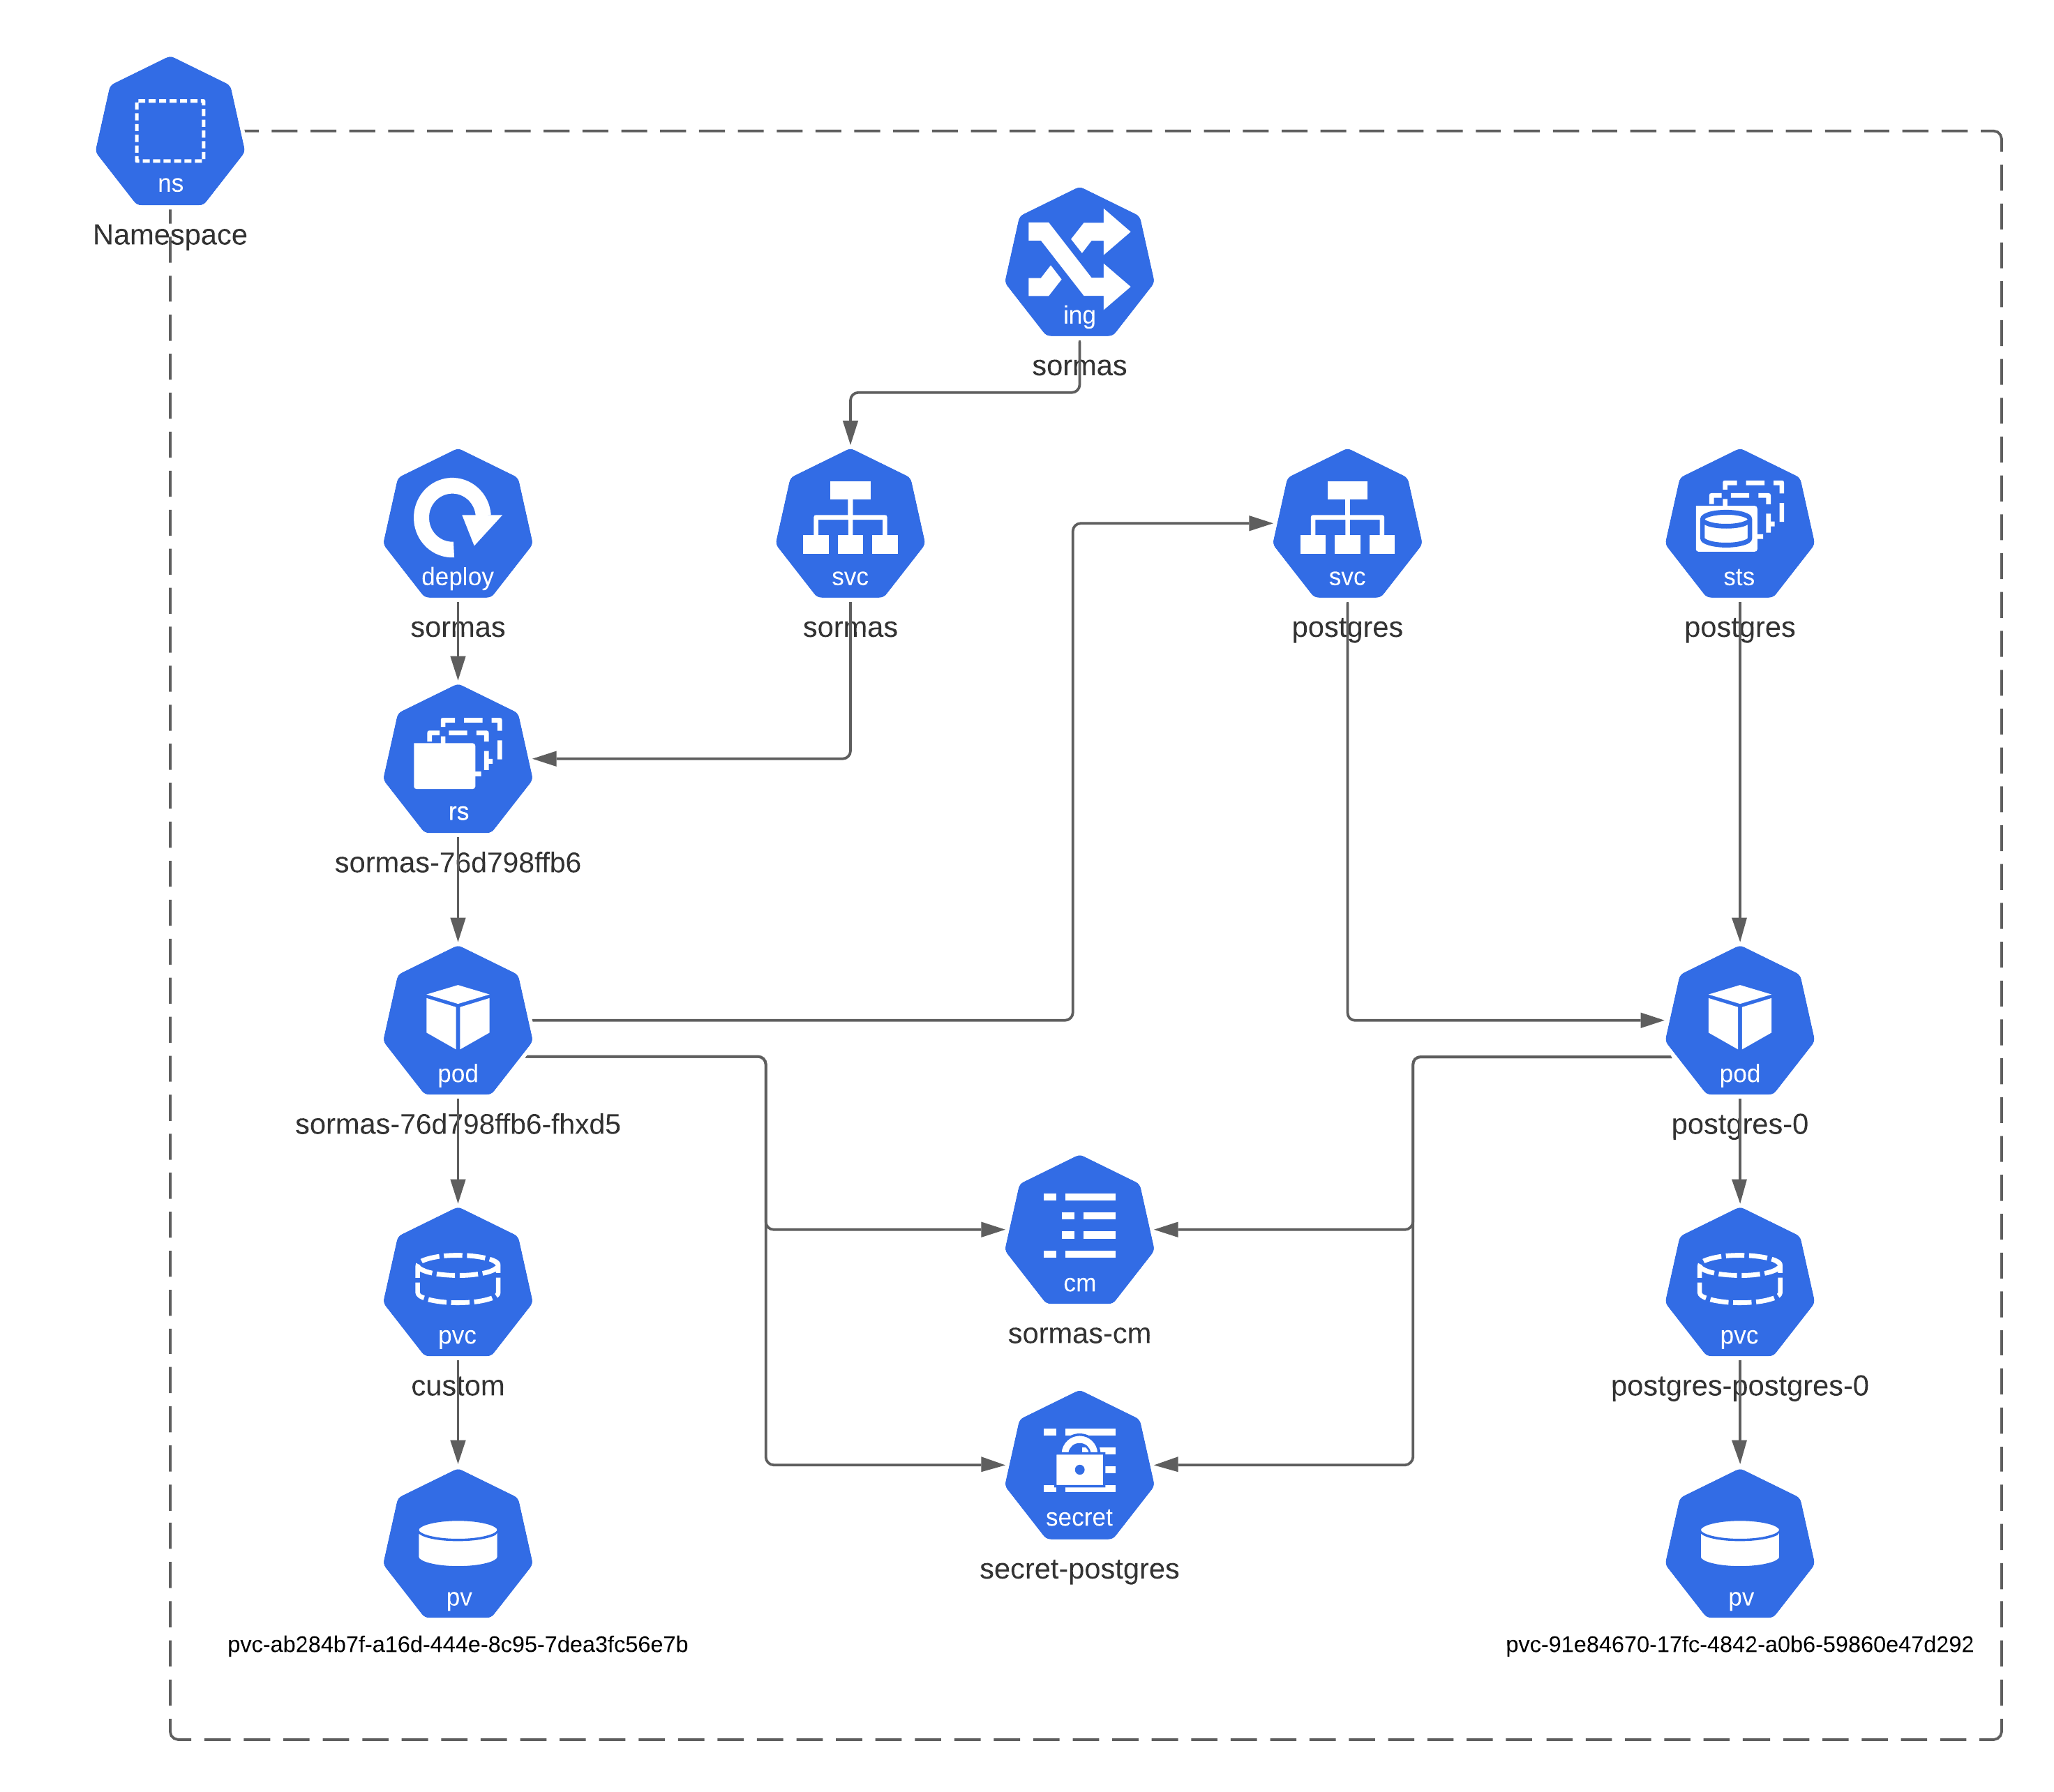
\includegraphics[width=\textwidth]{bilder/sormas_kubernetes.png}
\caption{SORMAS in Kubernetes}
\label{fig:sormas_kubernetes}
\end{figure}

Als Element zur Trennung und Organisation der einzelnen \ac{SORMAS}-Instanzen wird für jedes \ac{GA} ein eigener Namespace angelegt.
So kann jeder Pod genau einem \ac{GA} zugeordnet werden.\\
Wie zuvor angemerkt, ersetzt der Ingress an dieser Stelle den zuvor zur \ac{SSL}-Terminierung benötigten Apache2 Webserver.\\
Die Datenbank wird in einem StatefulSet ausgerollt, da diese durch die genaue Bestimmung der Pods besser persistent gestaltet werden kann.
Das StatefulSet erstellt dann seinen benötigten Pod, der über ein \ac{PVC} sein \ac{PV} zugeordnet bekommt. 
Die Konfiguration des Pods soll ausschließlich in der ConfigMap und dem Secret stattfinden, sodass nur an einer Stelle Anpassungen vorgenommen werden müssen.
Der Pod kann durch das Einrichtigen eins Services für andere Instanzen im selben Namespace erreichbar gemacht werden.\\
Der Payara-Server wird mit einem Deployment-Manifest ausgerollt. 
Die Eigenschaften des StatefulSets werden nicht benötigt und die Vorteile in Hinsicht auf das erleichterte Updaten der Software werden für zu erwartende Updates nützlich sein.
Das Deployment erstellt dann das entsprechende ReplicaSet und dieses den Pod. 
\ac{PV} und Konfiguration werden analog zu Postgres gemanaged. 
Der Service wählt mittels des Selectors allerdings das ReplicaSet und nicht den Pod selbst.


\subsection{Schreiben der Kubernetes Manifeste}



\section{Migration der Anwendung zur Kata-Runtime}


\subsection{Migration des Payara Servers}


\subsection{Migration der PostgreSQl-Datenbank}


\section{Helm Templating}